\documentclass{standalone}
\usepackage{tikz}
\usepackage{amsfonts}
\begin{document}
% Created by tikzDevice version 0.6.2-92-0ad2792 on 2013-03-02 14:56:50
% !TEX encoding = UTF-8 Unicode
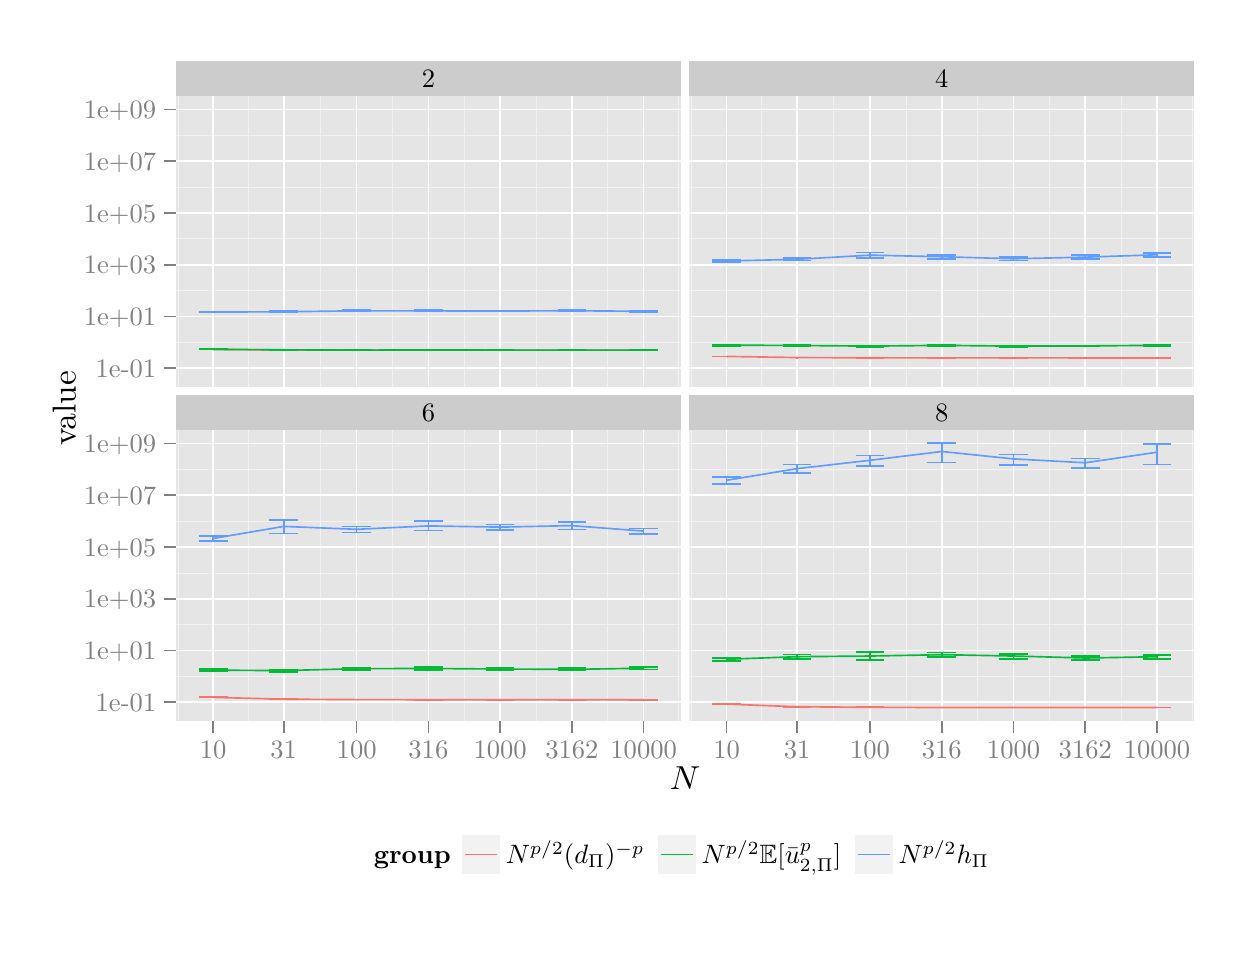
\begin{tikzpicture}[x=1pt,y=1pt]
\definecolor[named]{fillColor}{rgb}{1.00,1.00,1.00}
\path[use as bounding box,fill=fillColor,fill opacity=0.00] (0,0) rectangle (433.62,325.21);
\begin{scope}
\path[clip] (  0.00,  0.00) rectangle (433.62,325.21);
\definecolor[named]{drawColor}{rgb}{1.00,1.00,1.00}
\definecolor[named]{fillColor}{rgb}{1.00,1.00,1.00}

\path[draw=drawColor,line width= 0.6pt,line join=round,line cap=round,fill=fillColor] (  0.00,  0.00) rectangle (433.62,325.21);
\end{scope}
\begin{scope}
\path[clip] ( 53.55,195.47) rectangle (236.06,300.54);
\definecolor[named]{fillColor}{rgb}{0.90,0.90,0.90}

\path[fill=fillColor] ( 53.55,195.47) rectangle (236.06,300.54);
\definecolor[named]{drawColor}{rgb}{0.95,0.95,0.95}

\path[draw=drawColor,line width= 0.3pt,line join=round] ( 53.55,211.50) --
	(236.06,211.50);

\path[draw=drawColor,line width= 0.3pt,line join=round] ( 53.55,230.20) --
	(236.06,230.20);

\path[draw=drawColor,line width= 0.3pt,line join=round] ( 53.55,248.89) --
	(236.06,248.89);

\path[draw=drawColor,line width= 0.3pt,line join=round] ( 53.55,267.59) --
	(236.06,267.59);

\path[draw=drawColor,line width= 0.3pt,line join=round] ( 53.55,286.29) --
	(236.06,286.29);

\path[draw=drawColor,line width= 0.3pt,line join=round] ( 54.29,195.47) --
	( 54.29,300.54);

\path[draw=drawColor,line width= 0.3pt,line join=round] ( 79.77,195.47) --
	( 79.77,300.54);

\path[draw=drawColor,line width= 0.3pt,line join=round] (105.69,195.47) --
	(105.69,300.54);

\path[draw=drawColor,line width= 0.3pt,line join=round] (131.83,195.47) --
	(131.83,300.54);

\path[draw=drawColor,line width= 0.3pt,line join=round] (157.76,195.47) --
	(157.76,300.54);

\path[draw=drawColor,line width= 0.3pt,line join=round] (183.69,195.47) --
	(183.69,300.54);

\path[draw=drawColor,line width= 0.3pt,line join=round] (209.61,195.47) --
	(209.61,300.54);

\path[draw=drawColor,line width= 0.3pt,line join=round] (235.31,195.47) --
	(235.31,300.54);
\definecolor[named]{drawColor}{rgb}{1.00,1.00,1.00}

\path[draw=drawColor,line width= 0.6pt,line join=round] ( 53.55,202.15) --
	(236.06,202.15);

\path[draw=drawColor,line width= 0.6pt,line join=round] ( 53.55,220.85) --
	(236.06,220.85);

\path[draw=drawColor,line width= 0.6pt,line join=round] ( 53.55,239.55) --
	(236.06,239.55);

\path[draw=drawColor,line width= 0.6pt,line join=round] ( 53.55,258.24) --
	(236.06,258.24);

\path[draw=drawColor,line width= 0.6pt,line join=round] ( 53.55,276.94) --
	(236.06,276.94);

\path[draw=drawColor,line width= 0.6pt,line join=round] ( 53.55,295.63) --
	(236.06,295.63);

\path[draw=drawColor,line width= 0.6pt,line join=round] ( 67.03,195.47) --
	( 67.03,300.54);

\path[draw=drawColor,line width= 0.6pt,line join=round] ( 92.51,195.47) --
	( 92.51,300.54);

\path[draw=drawColor,line width= 0.6pt,line join=round] (118.88,195.47) --
	(118.88,300.54);

\path[draw=drawColor,line width= 0.6pt,line join=round] (144.79,195.47) --
	(144.79,300.54);

\path[draw=drawColor,line width= 0.6pt,line join=round] (170.73,195.47) --
	(170.73,300.54);

\path[draw=drawColor,line width= 0.6pt,line join=round] (196.65,195.47) --
	(196.65,300.54);

\path[draw=drawColor,line width= 0.6pt,line join=round] (222.58,195.47) --
	(222.58,300.54);
\definecolor[named]{drawColor}{rgb}{0.97,0.46,0.43}

\path[draw=drawColor,line width= 0.6pt,line join=round] ( 67.03,208.94) --
	( 92.51,208.76) --
	(118.88,208.71) --
	(144.79,208.69) --
	(170.73,208.69) --
	(196.65,208.69) --
	(222.58,208.69);
\definecolor[named]{drawColor}{rgb}{0.00,0.73,0.22}

\path[draw=drawColor,line width= 0.6pt,line join=round] ( 67.03,208.97) --
	( 92.51,208.80) --
	(118.88,208.68) --
	(144.79,208.76) --
	(170.73,208.69) --
	(196.65,208.68) --
	(222.58,208.68);
\definecolor[named]{drawColor}{rgb}{0.38,0.61,1.00}

\path[draw=drawColor,line width= 0.6pt,line join=round] ( 67.03,222.45) --
	( 92.51,222.54) --
	(118.88,222.89) --
	(144.79,222.87) --
	(170.73,222.81) --
	(196.65,222.92) --
	(222.58,222.71);
\definecolor[named]{drawColor}{rgb}{0.97,0.46,0.43}

\path[draw=drawColor,line width= 0.6pt,line join=round] ( 61.85,208.95) --
	( 72.22,208.95);

\path[draw=drawColor,line width= 0.6pt,line join=round] ( 67.03,208.95) --
	( 67.03,208.93);

\path[draw=drawColor,line width= 0.6pt,line join=round] ( 61.85,208.93) --
	( 72.22,208.93);

\path[draw=drawColor,line width= 0.6pt,line join=round] ( 87.32,208.76) --
	( 97.69,208.76);

\path[draw=drawColor,line width= 0.6pt,line join=round] ( 92.51,208.76) --
	( 92.51,208.76);

\path[draw=drawColor,line width= 0.6pt,line join=round] ( 87.32,208.76) --
	( 97.69,208.76);

\path[draw=drawColor,line width= 0.6pt,line join=round] (113.69,208.71) --
	(124.06,208.71);

\path[draw=drawColor,line width= 0.6pt,line join=round] (118.88,208.71) --
	(118.88,208.71);

\path[draw=drawColor,line width= 0.6pt,line join=round] (113.69,208.71) --
	(124.06,208.71);

\path[draw=drawColor,line width= 0.6pt,line join=round] (139.60,208.69) --
	(149.97,208.69);

\path[draw=drawColor,line width= 0.6pt,line join=round] (144.79,208.69) --
	(144.79,208.69);

\path[draw=drawColor,line width= 0.6pt,line join=round] (139.60,208.69) --
	(149.97,208.69);

\path[draw=drawColor,line width= 0.6pt,line join=round] (165.54,208.69) --
	(175.91,208.69);

\path[draw=drawColor,line width= 0.6pt,line join=round] (170.73,208.69) --
	(170.73,208.69);

\path[draw=drawColor,line width= 0.6pt,line join=round] (165.54,208.69) --
	(175.91,208.69);

\path[draw=drawColor,line width= 0.6pt,line join=round] (191.47,208.69) --
	(201.83,208.69);

\path[draw=drawColor,line width= 0.6pt,line join=round] (196.65,208.69) --
	(196.65,208.69);

\path[draw=drawColor,line width= 0.6pt,line join=round] (191.47,208.69) --
	(201.83,208.69);

\path[draw=drawColor,line width= 0.6pt,line join=round] (217.39,208.69) --
	(227.76,208.69);

\path[draw=drawColor,line width= 0.6pt,line join=round] (222.58,208.69) --
	(222.58,208.69);

\path[draw=drawColor,line width= 0.6pt,line join=round] (217.39,208.69) --
	(227.76,208.69);
\definecolor[named]{drawColor}{rgb}{0.00,0.73,0.22}

\path[draw=drawColor,line width= 0.6pt,line join=round] ( 61.85,209.08) --
	( 72.22,209.08);

\path[draw=drawColor,line width= 0.6pt,line join=round] ( 67.03,209.08) --
	( 67.03,208.87);

\path[draw=drawColor,line width= 0.6pt,line join=round] ( 61.85,208.87) --
	( 72.22,208.87);

\path[draw=drawColor,line width= 0.6pt,line join=round] ( 87.32,208.91) --
	( 97.69,208.91);

\path[draw=drawColor,line width= 0.6pt,line join=round] ( 92.51,208.91) --
	( 92.51,208.68);

\path[draw=drawColor,line width= 0.6pt,line join=round] ( 87.32,208.68) --
	( 97.69,208.68);

\path[draw=drawColor,line width= 0.6pt,line join=round] (113.69,208.79) --
	(124.06,208.79);

\path[draw=drawColor,line width= 0.6pt,line join=round] (118.88,208.79) --
	(118.88,208.56);

\path[draw=drawColor,line width= 0.6pt,line join=round] (113.69,208.56) --
	(124.06,208.56);

\path[draw=drawColor,line width= 0.6pt,line join=round] (139.60,208.87) --
	(149.97,208.87);

\path[draw=drawColor,line width= 0.6pt,line join=round] (144.79,208.87) --
	(144.79,208.64);

\path[draw=drawColor,line width= 0.6pt,line join=round] (139.60,208.64) --
	(149.97,208.64);

\path[draw=drawColor,line width= 0.6pt,line join=round] (165.54,208.80) --
	(175.91,208.80);

\path[draw=drawColor,line width= 0.6pt,line join=round] (170.73,208.80) --
	(170.73,208.57);

\path[draw=drawColor,line width= 0.6pt,line join=round] (165.54,208.57) --
	(175.91,208.57);

\path[draw=drawColor,line width= 0.6pt,line join=round] (191.47,208.80) --
	(201.83,208.80);

\path[draw=drawColor,line width= 0.6pt,line join=round] (196.65,208.80) --
	(196.65,208.56);

\path[draw=drawColor,line width= 0.6pt,line join=round] (191.47,208.56) --
	(201.83,208.56);

\path[draw=drawColor,line width= 0.6pt,line join=round] (217.39,208.80) --
	(227.76,208.80);

\path[draw=drawColor,line width= 0.6pt,line join=round] (222.58,208.80) --
	(222.58,208.56);

\path[draw=drawColor,line width= 0.6pt,line join=round] (217.39,208.56) --
	(227.76,208.56);
\definecolor[named]{drawColor}{rgb}{0.38,0.61,1.00}

\path[draw=drawColor,line width= 0.6pt,line join=round] ( 61.85,222.64) --
	( 72.22,222.64);

\path[draw=drawColor,line width= 0.6pt,line join=round] ( 67.03,222.64) --
	( 67.03,222.27);

\path[draw=drawColor,line width= 0.6pt,line join=round] ( 61.85,222.27) --
	( 72.22,222.27);

\path[draw=drawColor,line width= 0.6pt,line join=round] ( 87.32,222.76) --
	( 97.69,222.76);

\path[draw=drawColor,line width= 0.6pt,line join=round] ( 92.51,222.76) --
	( 92.51,222.34);

\path[draw=drawColor,line width= 0.6pt,line join=round] ( 87.32,222.34) --
	( 97.69,222.34);

\path[draw=drawColor,line width= 0.6pt,line join=round] (113.69,223.08) --
	(124.06,223.08);

\path[draw=drawColor,line width= 0.6pt,line join=round] (118.88,223.08) --
	(118.88,222.69);

\path[draw=drawColor,line width= 0.6pt,line join=round] (113.69,222.69) --
	(124.06,222.69);

\path[draw=drawColor,line width= 0.6pt,line join=round] (139.60,223.09) --
	(149.97,223.09);

\path[draw=drawColor,line width= 0.6pt,line join=round] (144.79,223.09) --
	(144.79,222.64);

\path[draw=drawColor,line width= 0.6pt,line join=round] (139.60,222.64) --
	(149.97,222.64);

\path[draw=drawColor,line width= 0.6pt,line join=round] (165.54,223.01) --
	(175.91,223.01);

\path[draw=drawColor,line width= 0.6pt,line join=round] (170.73,223.01) --
	(170.73,222.60);

\path[draw=drawColor,line width= 0.6pt,line join=round] (165.54,222.60) --
	(175.91,222.60);

\path[draw=drawColor,line width= 0.6pt,line join=round] (191.47,223.13) --
	(201.83,223.13);

\path[draw=drawColor,line width= 0.6pt,line join=round] (196.65,223.13) --
	(196.65,222.70);

\path[draw=drawColor,line width= 0.6pt,line join=round] (191.47,222.70) --
	(201.83,222.70);

\path[draw=drawColor,line width= 0.6pt,line join=round] (217.39,222.91) --
	(227.76,222.91);

\path[draw=drawColor,line width= 0.6pt,line join=round] (222.58,222.91) --
	(222.58,222.49);

\path[draw=drawColor,line width= 0.6pt,line join=round] (217.39,222.49) --
	(227.76,222.49);
\end{scope}
\begin{scope}
\path[clip] (239.07,195.47) rectangle (421.58,300.54);
\definecolor[named]{fillColor}{rgb}{0.90,0.90,0.90}

\path[fill=fillColor] (239.07,195.47) rectangle (421.57,300.54);
\definecolor[named]{drawColor}{rgb}{0.95,0.95,0.95}

\path[draw=drawColor,line width= 0.3pt,line join=round] (239.07,211.50) --
	(421.58,211.50);

\path[draw=drawColor,line width= 0.3pt,line join=round] (239.07,230.20) --
	(421.58,230.20);

\path[draw=drawColor,line width= 0.3pt,line join=round] (239.07,248.89) --
	(421.58,248.89);

\path[draw=drawColor,line width= 0.3pt,line join=round] (239.07,267.59) --
	(421.58,267.59);

\path[draw=drawColor,line width= 0.3pt,line join=round] (239.07,286.29) --
	(421.58,286.29);

\path[draw=drawColor,line width= 0.3pt,line join=round] (239.81,195.47) --
	(239.81,300.54);

\path[draw=drawColor,line width= 0.3pt,line join=round] (265.29,195.47) --
	(265.29,300.54);

\path[draw=drawColor,line width= 0.3pt,line join=round] (291.21,195.47) --
	(291.21,300.54);

\path[draw=drawColor,line width= 0.3pt,line join=round] (317.35,195.47) --
	(317.35,300.54);

\path[draw=drawColor,line width= 0.3pt,line join=round] (343.28,195.47) --
	(343.28,300.54);

\path[draw=drawColor,line width= 0.3pt,line join=round] (369.21,195.47) --
	(369.21,300.54);

\path[draw=drawColor,line width= 0.3pt,line join=round] (395.13,195.47) --
	(395.13,300.54);

\path[draw=drawColor,line width= 0.3pt,line join=round] (420.83,195.47) --
	(420.83,300.54);
\definecolor[named]{drawColor}{rgb}{1.00,1.00,1.00}

\path[draw=drawColor,line width= 0.6pt,line join=round] (239.07,202.15) --
	(421.58,202.15);

\path[draw=drawColor,line width= 0.6pt,line join=round] (239.07,220.85) --
	(421.58,220.85);

\path[draw=drawColor,line width= 0.6pt,line join=round] (239.07,239.55) --
	(421.58,239.55);

\path[draw=drawColor,line width= 0.6pt,line join=round] (239.07,258.24) --
	(421.58,258.24);

\path[draw=drawColor,line width= 0.6pt,line join=round] (239.07,276.94) --
	(421.58,276.94);

\path[draw=drawColor,line width= 0.6pt,line join=round] (239.07,295.63) --
	(421.58,295.63);

\path[draw=drawColor,line width= 0.6pt,line join=round] (252.55,195.47) --
	(252.55,300.54);

\path[draw=drawColor,line width= 0.6pt,line join=round] (278.03,195.47) --
	(278.03,300.54);

\path[draw=drawColor,line width= 0.6pt,line join=round] (304.40,195.47) --
	(304.40,300.54);

\path[draw=drawColor,line width= 0.6pt,line join=round] (330.31,195.47) --
	(330.31,300.54);

\path[draw=drawColor,line width= 0.6pt,line join=round] (356.25,195.47) --
	(356.25,300.54);

\path[draw=drawColor,line width= 0.6pt,line join=round] (382.17,195.47) --
	(382.17,300.54);

\path[draw=drawColor,line width= 0.6pt,line join=round] (408.09,195.47) --
	(408.09,300.54);
\definecolor[named]{drawColor}{rgb}{0.97,0.46,0.43}

\path[draw=drawColor,line width= 0.6pt,line join=round] (252.55,206.41) --
	(278.03,206.01) --
	(304.40,205.91) --
	(330.31,205.89) --
	(356.25,205.88) --
	(382.17,205.87) --
	(408.09,205.87);
\definecolor[named]{drawColor}{rgb}{0.00,0.73,0.22}

\path[draw=drawColor,line width= 0.6pt,line join=round] (252.55,210.48) --
	(278.03,210.37) --
	(304.40,210.14) --
	(330.31,210.40) --
	(356.25,210.14) --
	(382.17,210.21) --
	(408.09,210.41);
\definecolor[named]{drawColor}{rgb}{0.38,0.61,1.00}

\path[draw=drawColor,line width= 0.6pt,line join=round] (252.55,240.89) --
	(278.03,241.51) --
	(304.40,243.00) --
	(330.31,242.44) --
	(356.25,241.70) --
	(382.17,242.28) --
	(408.09,243.14);
\definecolor[named]{drawColor}{rgb}{0.97,0.46,0.43}

\path[draw=drawColor,line width= 0.6pt,line join=round] (247.36,206.43) --
	(257.73,206.43);

\path[draw=drawColor,line width= 0.6pt,line join=round] (252.55,206.43) --
	(252.55,206.39);

\path[draw=drawColor,line width= 0.6pt,line join=round] (247.36,206.39) --
	(257.73,206.39);

\path[draw=drawColor,line width= 0.6pt,line join=round] (272.84,206.02) --
	(283.21,206.02);

\path[draw=drawColor,line width= 0.6pt,line join=round] (278.03,206.02) --
	(278.03,206.01);

\path[draw=drawColor,line width= 0.6pt,line join=round] (272.84,206.01) --
	(283.21,206.01);

\path[draw=drawColor,line width= 0.6pt,line join=round] (299.21,205.92) --
	(309.58,205.92);

\path[draw=drawColor,line width= 0.6pt,line join=round] (304.40,205.92) --
	(304.40,205.91);

\path[draw=drawColor,line width= 0.6pt,line join=round] (299.21,205.91) --
	(309.58,205.91);

\path[draw=drawColor,line width= 0.6pt,line join=round] (325.12,205.89) --
	(335.49,205.89);

\path[draw=drawColor,line width= 0.6pt,line join=round] (330.31,205.89) --
	(330.31,205.89);

\path[draw=drawColor,line width= 0.6pt,line join=round] (325.12,205.89) --
	(335.49,205.89);

\path[draw=drawColor,line width= 0.6pt,line join=round] (351.06,205.88) --
	(361.43,205.88);

\path[draw=drawColor,line width= 0.6pt,line join=round] (356.25,205.88) --
	(356.25,205.88);

\path[draw=drawColor,line width= 0.6pt,line join=round] (351.06,205.88) --
	(361.43,205.88);

\path[draw=drawColor,line width= 0.6pt,line join=round] (376.98,205.87) --
	(387.35,205.87);

\path[draw=drawColor,line width= 0.6pt,line join=round] (382.17,205.87) --
	(382.17,205.87);

\path[draw=drawColor,line width= 0.6pt,line join=round] (376.98,205.87) --
	(387.35,205.87);

\path[draw=drawColor,line width= 0.6pt,line join=round] (402.91,205.87) --
	(413.28,205.87);

\path[draw=drawColor,line width= 0.6pt,line join=round] (408.09,205.87) --
	(408.09,205.87);

\path[draw=drawColor,line width= 0.6pt,line join=round] (402.91,205.87) --
	(413.28,205.87);
\definecolor[named]{drawColor}{rgb}{0.00,0.73,0.22}

\path[draw=drawColor,line width= 0.6pt,line join=round] (247.36,210.70) --
	(257.73,210.70);

\path[draw=drawColor,line width= 0.6pt,line join=round] (252.55,210.70) --
	(252.55,210.26);

\path[draw=drawColor,line width= 0.6pt,line join=round] (247.36,210.26) --
	(257.73,210.26);

\path[draw=drawColor,line width= 0.6pt,line join=round] (272.84,210.63) --
	(283.21,210.63);

\path[draw=drawColor,line width= 0.6pt,line join=round] (278.03,210.63) --
	(278.03,210.10);

\path[draw=drawColor,line width= 0.6pt,line join=round] (272.84,210.10) --
	(283.21,210.10);

\path[draw=drawColor,line width= 0.6pt,line join=round] (299.21,210.38) --
	(309.58,210.38);

\path[draw=drawColor,line width= 0.6pt,line join=round] (304.40,210.38) --
	(304.40,209.92);

\path[draw=drawColor,line width= 0.6pt,line join=round] (299.21,209.92) --
	(309.58,209.92);

\path[draw=drawColor,line width= 0.6pt,line join=round] (325.12,210.63) --
	(335.49,210.63);

\path[draw=drawColor,line width= 0.6pt,line join=round] (330.31,210.63) --
	(330.31,210.16);

\path[draw=drawColor,line width= 0.6pt,line join=round] (325.12,210.16) --
	(335.49,210.16);

\path[draw=drawColor,line width= 0.6pt,line join=round] (351.06,210.39) --
	(361.43,210.39);

\path[draw=drawColor,line width= 0.6pt,line join=round] (356.25,210.39) --
	(356.25,209.89);

\path[draw=drawColor,line width= 0.6pt,line join=round] (351.06,209.89) --
	(361.43,209.89);

\path[draw=drawColor,line width= 0.6pt,line join=round] (376.98,210.42) --
	(387.35,210.42);

\path[draw=drawColor,line width= 0.6pt,line join=round] (382.17,210.42) --
	(382.17,209.97);

\path[draw=drawColor,line width= 0.6pt,line join=round] (376.98,209.97) --
	(387.35,209.97);

\path[draw=drawColor,line width= 0.6pt,line join=round] (402.91,210.67) --
	(413.28,210.67);

\path[draw=drawColor,line width= 0.6pt,line join=round] (408.09,210.67) --
	(408.09,210.14);

\path[draw=drawColor,line width= 0.6pt,line join=round] (402.91,210.14) --
	(413.28,210.14);
\definecolor[named]{drawColor}{rgb}{0.38,0.61,1.00}

\path[draw=drawColor,line width= 0.6pt,line join=round] (247.36,241.28) --
	(257.73,241.28);

\path[draw=drawColor,line width= 0.6pt,line join=round] (252.55,241.28) --
	(252.55,240.52);

\path[draw=drawColor,line width= 0.6pt,line join=round] (247.36,240.52) --
	(257.73,240.52);

\path[draw=drawColor,line width= 0.6pt,line join=round] (272.84,241.97) --
	(283.21,241.97);

\path[draw=drawColor,line width= 0.6pt,line join=round] (278.03,241.97) --
	(278.03,241.05);

\path[draw=drawColor,line width= 0.6pt,line join=round] (272.84,241.05) --
	(283.21,241.05);

\path[draw=drawColor,line width= 0.6pt,line join=round] (299.21,243.92) --
	(309.58,243.92);

\path[draw=drawColor,line width= 0.6pt,line join=round] (304.40,243.92) --
	(304.40,242.04);

\path[draw=drawColor,line width= 0.6pt,line join=round] (299.21,242.04) --
	(309.58,242.04);

\path[draw=drawColor,line width= 0.6pt,line join=round] (325.12,243.17) --
	(335.49,243.17);

\path[draw=drawColor,line width= 0.6pt,line join=round] (330.31,243.17) --
	(330.31,241.69);

\path[draw=drawColor,line width= 0.6pt,line join=round] (325.12,241.69) --
	(335.49,241.69);

\path[draw=drawColor,line width= 0.6pt,line join=round] (351.06,242.28) --
	(361.43,242.28);

\path[draw=drawColor,line width= 0.6pt,line join=round] (356.25,242.28) --
	(356.25,241.08);

\path[draw=drawColor,line width= 0.6pt,line join=round] (351.06,241.08) --
	(361.43,241.08);

\path[draw=drawColor,line width= 0.6pt,line join=round] (376.98,242.97) --
	(387.35,242.97);

\path[draw=drawColor,line width= 0.6pt,line join=round] (382.17,242.97) --
	(382.17,241.63);

\path[draw=drawColor,line width= 0.6pt,line join=round] (376.98,241.63) --
	(387.35,241.63);

\path[draw=drawColor,line width= 0.6pt,line join=round] (402.91,243.85) --
	(413.28,243.85);

\path[draw=drawColor,line width= 0.6pt,line join=round] (408.09,243.85) --
	(408.09,242.35);

\path[draw=drawColor,line width= 0.6pt,line join=round] (402.91,242.35) --
	(413.28,242.35);
\end{scope}
\begin{scope}
\path[clip] ( 53.55, 74.76) rectangle (236.06,179.83);
\definecolor[named]{fillColor}{rgb}{0.90,0.90,0.90}

\path[fill=fillColor] ( 53.55, 74.76) rectangle (236.06,179.83);
\definecolor[named]{drawColor}{rgb}{0.95,0.95,0.95}

\path[draw=drawColor,line width= 0.3pt,line join=round] ( 53.55, 90.79) --
	(236.06, 90.79);

\path[draw=drawColor,line width= 0.3pt,line join=round] ( 53.55,109.49) --
	(236.06,109.49);

\path[draw=drawColor,line width= 0.3pt,line join=round] ( 53.55,128.18) --
	(236.06,128.18);

\path[draw=drawColor,line width= 0.3pt,line join=round] ( 53.55,146.88) --
	(236.06,146.88);

\path[draw=drawColor,line width= 0.3pt,line join=round] ( 53.55,165.57) --
	(236.06,165.57);

\path[draw=drawColor,line width= 0.3pt,line join=round] ( 54.29, 74.76) --
	( 54.29,179.83);

\path[draw=drawColor,line width= 0.3pt,line join=round] ( 79.77, 74.76) --
	( 79.77,179.83);

\path[draw=drawColor,line width= 0.3pt,line join=round] (105.69, 74.76) --
	(105.69,179.83);

\path[draw=drawColor,line width= 0.3pt,line join=round] (131.83, 74.76) --
	(131.83,179.83);

\path[draw=drawColor,line width= 0.3pt,line join=round] (157.76, 74.76) --
	(157.76,179.83);

\path[draw=drawColor,line width= 0.3pt,line join=round] (183.69, 74.76) --
	(183.69,179.83);

\path[draw=drawColor,line width= 0.3pt,line join=round] (209.61, 74.76) --
	(209.61,179.83);

\path[draw=drawColor,line width= 0.3pt,line join=round] (235.31, 74.76) --
	(235.31,179.83);
\definecolor[named]{drawColor}{rgb}{1.00,1.00,1.00}

\path[draw=drawColor,line width= 0.6pt,line join=round] ( 53.55, 81.44) --
	(236.06, 81.44);

\path[draw=drawColor,line width= 0.6pt,line join=round] ( 53.55,100.14) --
	(236.06,100.14);

\path[draw=drawColor,line width= 0.6pt,line join=round] ( 53.55,118.83) --
	(236.06,118.83);

\path[draw=drawColor,line width= 0.6pt,line join=round] ( 53.55,137.53) --
	(236.06,137.53);

\path[draw=drawColor,line width= 0.6pt,line join=round] ( 53.55,156.23) --
	(236.06,156.23);

\path[draw=drawColor,line width= 0.6pt,line join=round] ( 53.55,174.92) --
	(236.06,174.92);

\path[draw=drawColor,line width= 0.6pt,line join=round] ( 67.03, 74.76) --
	( 67.03,179.83);

\path[draw=drawColor,line width= 0.6pt,line join=round] ( 92.51, 74.76) --
	( 92.51,179.83);

\path[draw=drawColor,line width= 0.6pt,line join=round] (118.88, 74.76) --
	(118.88,179.83);

\path[draw=drawColor,line width= 0.6pt,line join=round] (144.79, 74.76) --
	(144.79,179.83);

\path[draw=drawColor,line width= 0.6pt,line join=round] (170.73, 74.76) --
	(170.73,179.83);

\path[draw=drawColor,line width= 0.6pt,line join=round] (196.65, 74.76) --
	(196.65,179.83);

\path[draw=drawColor,line width= 0.6pt,line join=round] (222.58, 74.76) --
	(222.58,179.83);
\definecolor[named]{drawColor}{rgb}{0.97,0.46,0.43}

\path[draw=drawColor,line width= 0.6pt,line join=round] ( 67.03, 83.21) --
	( 92.51, 82.56) --
	(118.88, 82.41) --
	(144.79, 82.37) --
	(170.73, 82.36) --
	(196.65, 82.35) --
	(222.58, 82.35);
\definecolor[named]{drawColor}{rgb}{0.00,0.73,0.22}

\path[draw=drawColor,line width= 0.6pt,line join=round] ( 67.03, 93.04) --
	( 92.51, 92.89) --
	(118.88, 93.58) --
	(144.79, 93.65) --
	(170.73, 93.46) --
	(196.65, 93.33) --
	(222.58, 93.75);
\definecolor[named]{drawColor}{rgb}{0.38,0.61,1.00}

\path[draw=drawColor,line width= 0.6pt,line join=round] ( 67.03,140.63) --
	( 92.51,144.99) --
	(118.88,143.94) --
	(144.79,145.17) --
	(170.73,144.74) --
	(196.65,145.27) --
	(222.58,143.29);
\definecolor[named]{drawColor}{rgb}{0.97,0.46,0.43}

\path[draw=drawColor,line width= 0.6pt,line join=round] ( 61.85, 83.24) --
	( 72.22, 83.24);

\path[draw=drawColor,line width= 0.6pt,line join=round] ( 67.03, 83.24) --
	( 67.03, 83.17);

\path[draw=drawColor,line width= 0.6pt,line join=round] ( 61.85, 83.17) --
	( 72.22, 83.17);

\path[draw=drawColor,line width= 0.6pt,line join=round] ( 87.32, 82.56) --
	( 97.69, 82.56);

\path[draw=drawColor,line width= 0.6pt,line join=round] ( 92.51, 82.56) --
	( 92.51, 82.55);

\path[draw=drawColor,line width= 0.6pt,line join=round] ( 87.32, 82.55) --
	( 97.69, 82.55);

\path[draw=drawColor,line width= 0.6pt,line join=round] (113.69, 82.41) --
	(124.06, 82.41);

\path[draw=drawColor,line width= 0.6pt,line join=round] (118.88, 82.41) --
	(118.88, 82.41);

\path[draw=drawColor,line width= 0.6pt,line join=round] (113.69, 82.41) --
	(124.06, 82.41);

\path[draw=drawColor,line width= 0.6pt,line join=round] (139.60, 82.37) --
	(149.97, 82.37);

\path[draw=drawColor,line width= 0.6pt,line join=round] (144.79, 82.37) --
	(144.79, 82.37);

\path[draw=drawColor,line width= 0.6pt,line join=round] (139.60, 82.37) --
	(149.97, 82.37);

\path[draw=drawColor,line width= 0.6pt,line join=round] (165.54, 82.36) --
	(175.91, 82.36);

\path[draw=drawColor,line width= 0.6pt,line join=round] (170.73, 82.36) --
	(170.73, 82.35);

\path[draw=drawColor,line width= 0.6pt,line join=round] (165.54, 82.35) --
	(175.91, 82.35);

\path[draw=drawColor,line width= 0.6pt,line join=round] (191.47, 82.35) --
	(201.83, 82.35);

\path[draw=drawColor,line width= 0.6pt,line join=round] (196.65, 82.35) --
	(196.65, 82.35);

\path[draw=drawColor,line width= 0.6pt,line join=round] (191.47, 82.35) --
	(201.83, 82.35);

\path[draw=drawColor,line width= 0.6pt,line join=round] (217.39, 82.35) --
	(227.76, 82.35);

\path[draw=drawColor,line width= 0.6pt,line join=round] (222.58, 82.35) --
	(222.58, 82.35);

\path[draw=drawColor,line width= 0.6pt,line join=round] (217.39, 82.35) --
	(227.76, 82.35);
\definecolor[named]{drawColor}{rgb}{0.00,0.73,0.22}

\path[draw=drawColor,line width= 0.6pt,line join=round] ( 61.85, 93.39) --
	( 72.22, 93.39);

\path[draw=drawColor,line width= 0.6pt,line join=round] ( 67.03, 93.39) --
	( 67.03, 92.66);

\path[draw=drawColor,line width= 0.6pt,line join=round] ( 61.85, 92.66) --
	( 72.22, 92.66);

\path[draw=drawColor,line width= 0.6pt,line join=round] ( 87.32, 93.32) --
	( 97.69, 93.32);

\path[draw=drawColor,line width= 0.6pt,line join=round] ( 92.51, 93.32) --
	( 92.51, 92.47);

\path[draw=drawColor,line width= 0.6pt,line join=round] ( 87.32, 92.47) --
	( 97.69, 92.47);

\path[draw=drawColor,line width= 0.6pt,line join=round] (113.69, 94.01) --
	(124.06, 94.01);

\path[draw=drawColor,line width= 0.6pt,line join=round] (118.88, 94.01) --
	(118.88, 93.10);

\path[draw=drawColor,line width= 0.6pt,line join=round] (113.69, 93.10) --
	(124.06, 93.10);

\path[draw=drawColor,line width= 0.6pt,line join=round] (139.60, 94.21) --
	(149.97, 94.21);

\path[draw=drawColor,line width= 0.6pt,line join=round] (144.79, 94.21) --
	(144.79, 93.05);

\path[draw=drawColor,line width= 0.6pt,line join=round] (139.60, 93.05) --
	(149.97, 93.05);

\path[draw=drawColor,line width= 0.6pt,line join=round] (165.54, 93.92) --
	(175.91, 93.92);

\path[draw=drawColor,line width= 0.6pt,line join=round] (170.73, 93.92) --
	(170.73, 93.00);

\path[draw=drawColor,line width= 0.6pt,line join=round] (165.54, 93.00) --
	(175.91, 93.00);

\path[draw=drawColor,line width= 0.6pt,line join=round] (191.47, 93.75) --
	(201.83, 93.75);

\path[draw=drawColor,line width= 0.6pt,line join=round] (196.65, 93.75) --
	(196.65, 92.91);

\path[draw=drawColor,line width= 0.6pt,line join=round] (191.47, 92.91) --
	(201.83, 92.91);

\path[draw=drawColor,line width= 0.6pt,line join=round] (217.39, 94.17) --
	(227.76, 94.17);

\path[draw=drawColor,line width= 0.6pt,line join=round] (222.58, 94.17) --
	(222.58, 93.30);

\path[draw=drawColor,line width= 0.6pt,line join=round] (217.39, 93.30) --
	(227.76, 93.30);
\definecolor[named]{drawColor}{rgb}{0.38,0.61,1.00}

\path[draw=drawColor,line width= 0.6pt,line join=round] ( 61.85,141.41) --
	( 72.22,141.41);

\path[draw=drawColor,line width= 0.6pt,line join=round] ( 67.03,141.41) --
	( 67.03,139.79);

\path[draw=drawColor,line width= 0.6pt,line join=round] ( 61.85,139.79) --
	( 72.22,139.79);

\path[draw=drawColor,line width= 0.6pt,line join=round] ( 87.32,147.23) --
	( 97.69,147.23);

\path[draw=drawColor,line width= 0.6pt,line join=round] ( 92.51,147.23) --
	( 92.51,142.39);

\path[draw=drawColor,line width= 0.6pt,line join=round] ( 87.32,142.39) --
	( 97.69,142.39);

\path[draw=drawColor,line width= 0.6pt,line join=round] (113.69,144.97) --
	(124.06,144.97);

\path[draw=drawColor,line width= 0.6pt,line join=round] (118.88,144.97) --
	(118.88,142.80);

\path[draw=drawColor,line width= 0.6pt,line join=round] (113.69,142.80) --
	(124.06,142.80);

\path[draw=drawColor,line width= 0.6pt,line join=round] (139.60,146.93) --
	(149.97,146.93);

\path[draw=drawColor,line width= 0.6pt,line join=round] (144.79,146.93) --
	(144.79,143.48);

\path[draw=drawColor,line width= 0.6pt,line join=round] (139.60,143.48) --
	(149.97,143.48);

\path[draw=drawColor,line width= 0.6pt,line join=round] (165.54,145.65) --
	(175.91,145.65);

\path[draw=drawColor,line width= 0.6pt,line join=round] (170.73,145.65) --
	(170.73,143.68);

\path[draw=drawColor,line width= 0.6pt,line join=round] (165.54,143.68) --
	(175.91,143.68);

\path[draw=drawColor,line width= 0.6pt,line join=round] (191.47,146.64) --
	(201.83,146.64);

\path[draw=drawColor,line width= 0.6pt,line join=round] (196.65,146.64) --
	(196.65,143.82);

\path[draw=drawColor,line width= 0.6pt,line join=round] (191.47,143.82) --
	(201.83,143.82);

\path[draw=drawColor,line width= 0.6pt,line join=round] (217.39,144.20) --
	(227.76,144.20);

\path[draw=drawColor,line width= 0.6pt,line join=round] (222.58,144.20) --
	(222.58,142.23);

\path[draw=drawColor,line width= 0.6pt,line join=round] (217.39,142.23) --
	(227.76,142.23);
\end{scope}
\begin{scope}
\path[clip] (239.07, 74.76) rectangle (421.58,179.83);
\definecolor[named]{fillColor}{rgb}{0.90,0.90,0.90}

\path[fill=fillColor] (239.07, 74.76) rectangle (421.57,179.83);
\definecolor[named]{drawColor}{rgb}{0.95,0.95,0.95}

\path[draw=drawColor,line width= 0.3pt,line join=round] (239.07, 90.79) --
	(421.58, 90.79);

\path[draw=drawColor,line width= 0.3pt,line join=round] (239.07,109.49) --
	(421.58,109.49);

\path[draw=drawColor,line width= 0.3pt,line join=round] (239.07,128.18) --
	(421.58,128.18);

\path[draw=drawColor,line width= 0.3pt,line join=round] (239.07,146.88) --
	(421.58,146.88);

\path[draw=drawColor,line width= 0.3pt,line join=round] (239.07,165.57) --
	(421.58,165.57);

\path[draw=drawColor,line width= 0.3pt,line join=round] (239.81, 74.76) --
	(239.81,179.83);

\path[draw=drawColor,line width= 0.3pt,line join=round] (265.29, 74.76) --
	(265.29,179.83);

\path[draw=drawColor,line width= 0.3pt,line join=round] (291.21, 74.76) --
	(291.21,179.83);

\path[draw=drawColor,line width= 0.3pt,line join=round] (317.35, 74.76) --
	(317.35,179.83);

\path[draw=drawColor,line width= 0.3pt,line join=round] (343.28, 74.76) --
	(343.28,179.83);

\path[draw=drawColor,line width= 0.3pt,line join=round] (369.21, 74.76) --
	(369.21,179.83);

\path[draw=drawColor,line width= 0.3pt,line join=round] (395.13, 74.76) --
	(395.13,179.83);

\path[draw=drawColor,line width= 0.3pt,line join=round] (420.83, 74.76) --
	(420.83,179.83);
\definecolor[named]{drawColor}{rgb}{1.00,1.00,1.00}

\path[draw=drawColor,line width= 0.6pt,line join=round] (239.07, 81.44) --
	(421.58, 81.44);

\path[draw=drawColor,line width= 0.6pt,line join=round] (239.07,100.14) --
	(421.58,100.14);

\path[draw=drawColor,line width= 0.6pt,line join=round] (239.07,118.83) --
	(421.58,118.83);

\path[draw=drawColor,line width= 0.6pt,line join=round] (239.07,137.53) --
	(421.58,137.53);

\path[draw=drawColor,line width= 0.6pt,line join=round] (239.07,156.23) --
	(421.58,156.23);

\path[draw=drawColor,line width= 0.6pt,line join=round] (239.07,174.92) --
	(421.58,174.92);

\path[draw=drawColor,line width= 0.6pt,line join=round] (252.55, 74.76) --
	(252.55,179.83);

\path[draw=drawColor,line width= 0.6pt,line join=round] (278.03, 74.76) --
	(278.03,179.83);

\path[draw=drawColor,line width= 0.6pt,line join=round] (304.40, 74.76) --
	(304.40,179.83);

\path[draw=drawColor,line width= 0.6pt,line join=round] (330.31, 74.76) --
	(330.31,179.83);

\path[draw=drawColor,line width= 0.6pt,line join=round] (356.25, 74.76) --
	(356.25,179.83);

\path[draw=drawColor,line width= 0.6pt,line join=round] (382.17, 74.76) --
	(382.17,179.83);

\path[draw=drawColor,line width= 0.6pt,line join=round] (408.09, 74.76) --
	(408.09,179.83);
\definecolor[named]{drawColor}{rgb}{0.97,0.46,0.43}

\path[draw=drawColor,line width= 0.6pt,line join=round] (252.55, 80.77) --
	(278.03, 79.83) --
	(304.40, 79.62) --
	(330.31, 79.56) --
	(356.25, 79.54) --
	(382.17, 79.54) --
	(408.09, 79.54);
\definecolor[named]{drawColor}{rgb}{0.00,0.73,0.22}

\path[draw=drawColor,line width= 0.6pt,line join=round] (252.55, 96.99) --
	(278.03, 97.91) --
	(304.40, 98.15) --
	(330.31, 98.64) --
	(356.25, 98.15) --
	(382.17, 97.44) --
	(408.09, 97.89);
\definecolor[named]{drawColor}{rgb}{0.38,0.61,1.00}

\path[draw=drawColor,line width= 0.6pt,line join=round] (252.55,161.65) --
	(278.03,165.87) --
	(304.40,168.88) --
	(330.31,172.06) --
	(356.25,169.38) --
	(382.17,167.98) --
	(408.09,171.80);
\definecolor[named]{drawColor}{rgb}{0.97,0.46,0.43}

\path[draw=drawColor,line width= 0.6pt,line join=round] (247.36, 80.83) --
	(257.73, 80.83);

\path[draw=drawColor,line width= 0.6pt,line join=round] (252.55, 80.83) --
	(252.55, 80.71);

\path[draw=drawColor,line width= 0.6pt,line join=round] (247.36, 80.71) --
	(257.73, 80.71);

\path[draw=drawColor,line width= 0.6pt,line join=round] (272.84, 79.84) --
	(283.21, 79.84);

\path[draw=drawColor,line width= 0.6pt,line join=round] (278.03, 79.84) --
	(278.03, 79.82);

\path[draw=drawColor,line width= 0.6pt,line join=round] (272.84, 79.82) --
	(283.21, 79.82);

\path[draw=drawColor,line width= 0.6pt,line join=round] (299.21, 79.62) --
	(309.58, 79.62);

\path[draw=drawColor,line width= 0.6pt,line join=round] (304.40, 79.62) --
	(304.40, 79.61);

\path[draw=drawColor,line width= 0.6pt,line join=round] (299.21, 79.61) --
	(309.58, 79.61);

\path[draw=drawColor,line width= 0.6pt,line join=round] (325.12, 79.56) --
	(335.49, 79.56);

\path[draw=drawColor,line width= 0.6pt,line join=round] (330.31, 79.56) --
	(330.31, 79.56);

\path[draw=drawColor,line width= 0.6pt,line join=round] (325.12, 79.56) --
	(335.49, 79.56);

\path[draw=drawColor,line width= 0.6pt,line join=round] (351.06, 79.54) --
	(361.43, 79.54);

\path[draw=drawColor,line width= 0.6pt,line join=round] (356.25, 79.54) --
	(356.25, 79.54);

\path[draw=drawColor,line width= 0.6pt,line join=round] (351.06, 79.54) --
	(361.43, 79.54);

\path[draw=drawColor,line width= 0.6pt,line join=round] (376.98, 79.54) --
	(387.35, 79.54);

\path[draw=drawColor,line width= 0.6pt,line join=round] (382.17, 79.54) --
	(382.17, 79.54);

\path[draw=drawColor,line width= 0.6pt,line join=round] (376.98, 79.54) --
	(387.35, 79.54);

\path[draw=drawColor,line width= 0.6pt,line join=round] (402.91, 79.54) --
	(413.28, 79.54);

\path[draw=drawColor,line width= 0.6pt,line join=round] (408.09, 79.54) --
	(408.09, 79.54);

\path[draw=drawColor,line width= 0.6pt,line join=round] (402.91, 79.54) --
	(413.28, 79.54);
\definecolor[named]{drawColor}{rgb}{0.00,0.73,0.22}

\path[draw=drawColor,line width= 0.6pt,line join=round] (247.36, 97.55) --
	(257.73, 97.55);

\path[draw=drawColor,line width= 0.6pt,line join=round] (252.55, 97.55) --
	(252.55, 96.43);

\path[draw=drawColor,line width= 0.6pt,line join=round] (247.36, 96.43) --
	(257.73, 96.43);

\path[draw=drawColor,line width= 0.6pt,line join=round] (272.84, 98.72) --
	(283.21, 98.72);

\path[draw=drawColor,line width= 0.6pt,line join=round] (278.03, 98.72) --
	(278.03, 97.03);

\path[draw=drawColor,line width= 0.6pt,line join=round] (272.84, 97.03) --
	(283.21, 97.03);

\path[draw=drawColor,line width= 0.6pt,line join=round] (299.21, 99.51) --
	(309.58, 99.51);

\path[draw=drawColor,line width= 0.6pt,line join=round] (304.40, 99.51) --
	(304.40, 96.79);

\path[draw=drawColor,line width= 0.6pt,line join=round] (299.21, 96.79) --
	(309.58, 96.79);

\path[draw=drawColor,line width= 0.6pt,line join=round] (325.12, 99.45) --
	(335.49, 99.45);

\path[draw=drawColor,line width= 0.6pt,line join=round] (330.31, 99.45) --
	(330.31, 97.76);

\path[draw=drawColor,line width= 0.6pt,line join=round] (325.12, 97.76) --
	(335.49, 97.76);

\path[draw=drawColor,line width= 0.6pt,line join=round] (351.06, 98.97) --
	(361.43, 98.97);

\path[draw=drawColor,line width= 0.6pt,line join=round] (356.25, 98.97) --
	(356.25, 97.17);

\path[draw=drawColor,line width= 0.6pt,line join=round] (351.06, 97.17) --
	(361.43, 97.17);

\path[draw=drawColor,line width= 0.6pt,line join=round] (376.98, 98.12) --
	(387.35, 98.12);

\path[draw=drawColor,line width= 0.6pt,line join=round] (382.17, 98.12) --
	(382.17, 96.74);

\path[draw=drawColor,line width= 0.6pt,line join=round] (376.98, 96.74) --
	(387.35, 96.74);

\path[draw=drawColor,line width= 0.6pt,line join=round] (402.91, 98.64) --
	(413.28, 98.64);

\path[draw=drawColor,line width= 0.6pt,line join=round] (408.09, 98.64) --
	(408.09, 97.09);

\path[draw=drawColor,line width= 0.6pt,line join=round] (402.91, 97.09) --
	(413.28, 97.09);
\definecolor[named]{drawColor}{rgb}{0.38,0.61,1.00}

\path[draw=drawColor,line width= 0.6pt,line join=round] (247.36,162.77) --
	(257.73,162.77);

\path[draw=drawColor,line width= 0.6pt,line join=round] (252.55,162.77) --
	(252.55,160.25);

\path[draw=drawColor,line width= 0.6pt,line join=round] (247.36,160.25) --
	(257.73,160.25);

\path[draw=drawColor,line width= 0.6pt,line join=round] (272.84,167.33) --
	(283.21,167.33);

\path[draw=drawColor,line width= 0.6pt,line join=round] (278.03,167.33) --
	(278.03,164.20);

\path[draw=drawColor,line width= 0.6pt,line join=round] (272.84,164.20) --
	(283.21,164.20);

\path[draw=drawColor,line width= 0.6pt,line join=round] (299.21,170.59) --
	(309.58,170.59);

\path[draw=drawColor,line width= 0.6pt,line join=round] (304.40,170.59) --
	(304.40,166.79);

\path[draw=drawColor,line width= 0.6pt,line join=round] (299.21,166.79) --
	(309.58,166.79);

\path[draw=drawColor,line width= 0.6pt,line join=round] (325.12,175.05) --
	(335.49,175.05);

\path[draw=drawColor,line width= 0.6pt,line join=round] (330.31,175.05) --
	(330.31,168.04);

\path[draw=drawColor,line width= 0.6pt,line join=round] (325.12,168.04) --
	(335.49,168.04);

\path[draw=drawColor,line width= 0.6pt,line join=round] (351.06,170.99) --
	(361.43,170.99);

\path[draw=drawColor,line width= 0.6pt,line join=round] (356.25,170.99) --
	(356.25,167.15);

\path[draw=drawColor,line width= 0.6pt,line join=round] (351.06,167.15) --
	(361.43,167.15);

\path[draw=drawColor,line width= 0.6pt,line join=round] (376.98,169.51) --
	(387.35,169.51);

\path[draw=drawColor,line width= 0.6pt,line join=round] (382.17,169.51) --
	(382.17,166.21);

\path[draw=drawColor,line width= 0.6pt,line join=round] (376.98,166.21) --
	(387.35,166.21);

\path[draw=drawColor,line width= 0.6pt,line join=round] (402.91,174.81) --
	(413.28,174.81);

\path[draw=drawColor,line width= 0.6pt,line join=round] (408.09,174.81) --
	(408.09,167.41);

\path[draw=drawColor,line width= 0.6pt,line join=round] (402.91,167.41) --
	(413.28,167.41);
\end{scope}
\begin{scope}
\path[clip] (  0.00,  0.00) rectangle (433.62,325.21);
\definecolor[named]{fillColor}{rgb}{0.80,0.80,0.80}

\path[fill=fillColor] ( 53.55,300.54) rectangle (236.06,313.17);
\definecolor[named]{drawColor}{rgb}{0.00,0.00,0.00}

\node[text=drawColor,anchor=base,inner sep=0pt, outer sep=0pt, scale=  0.96] at (144.80,303.55) {2};
\end{scope}
\begin{scope}
\path[clip] (  0.00,  0.00) rectangle (433.62,325.21);
\definecolor[named]{fillColor}{rgb}{0.80,0.80,0.80}

\path[fill=fillColor] (239.07,300.54) rectangle (421.57,313.17);
\definecolor[named]{drawColor}{rgb}{0.00,0.00,0.00}

\node[text=drawColor,anchor=base,inner sep=0pt, outer sep=0pt, scale=  0.96] at (330.32,303.55) {4};
\end{scope}
\begin{scope}
\path[clip] (  0.00,  0.00) rectangle (433.62,325.21);
\definecolor[named]{fillColor}{rgb}{0.80,0.80,0.80}

\path[fill=fillColor] ( 53.55,179.83) rectangle (236.06,192.46);
\definecolor[named]{drawColor}{rgb}{0.00,0.00,0.00}

\node[text=drawColor,anchor=base,inner sep=0pt, outer sep=0pt, scale=  0.96] at (144.80,182.84) {6};
\end{scope}
\begin{scope}
\path[clip] (  0.00,  0.00) rectangle (433.62,325.21);
\definecolor[named]{fillColor}{rgb}{0.80,0.80,0.80}

\path[fill=fillColor] (239.07,179.83) rectangle (421.57,192.46);
\definecolor[named]{drawColor}{rgb}{0.00,0.00,0.00}

\node[text=drawColor,anchor=base,inner sep=0pt, outer sep=0pt, scale=  0.96] at (330.32,182.84) {8};
\end{scope}
\begin{scope}
\path[clip] (  0.00,  0.00) rectangle (433.62,325.21);
\definecolor[named]{drawColor}{rgb}{0.50,0.50,0.50}

\node[text=drawColor,anchor=base east,inner sep=0pt, outer sep=0pt, scale=  0.96] at ( 46.44,198.85) {1e-01};

\node[text=drawColor,anchor=base east,inner sep=0pt, outer sep=0pt, scale=  0.96] at ( 46.44,217.54) {1e+01};

\node[text=drawColor,anchor=base east,inner sep=0pt, outer sep=0pt, scale=  0.96] at ( 46.44,236.24) {1e+03};

\node[text=drawColor,anchor=base east,inner sep=0pt, outer sep=0pt, scale=  0.96] at ( 46.44,254.94) {1e+05};

\node[text=drawColor,anchor=base east,inner sep=0pt, outer sep=0pt, scale=  0.96] at ( 46.44,273.63) {1e+07};

\node[text=drawColor,anchor=base east,inner sep=0pt, outer sep=0pt, scale=  0.96] at ( 46.44,292.33) {1e+09};
\end{scope}
\begin{scope}
\path[clip] (  0.00,  0.00) rectangle (433.62,325.21);
\definecolor[named]{drawColor}{rgb}{0.50,0.50,0.50}

\path[draw=drawColor,line width= 0.6pt,line join=round] ( 49.28,202.15) --
	( 53.55,202.15);

\path[draw=drawColor,line width= 0.6pt,line join=round] ( 49.28,220.85) --
	( 53.55,220.85);

\path[draw=drawColor,line width= 0.6pt,line join=round] ( 49.28,239.55) --
	( 53.55,239.55);

\path[draw=drawColor,line width= 0.6pt,line join=round] ( 49.28,258.24) --
	( 53.55,258.24);

\path[draw=drawColor,line width= 0.6pt,line join=round] ( 49.28,276.94) --
	( 53.55,276.94);

\path[draw=drawColor,line width= 0.6pt,line join=round] ( 49.28,295.63) --
	( 53.55,295.63);
\end{scope}
\begin{scope}
\path[clip] (  0.00,  0.00) rectangle (433.62,325.21);
\definecolor[named]{drawColor}{rgb}{0.50,0.50,0.50}

\node[text=drawColor,anchor=base east,inner sep=0pt, outer sep=0pt, scale=  0.96] at ( 46.44, 78.14) {1e-01};

\node[text=drawColor,anchor=base east,inner sep=0pt, outer sep=0pt, scale=  0.96] at ( 46.44, 96.83) {1e+01};

\node[text=drawColor,anchor=base east,inner sep=0pt, outer sep=0pt, scale=  0.96] at ( 46.44,115.53) {1e+03};

\node[text=drawColor,anchor=base east,inner sep=0pt, outer sep=0pt, scale=  0.96] at ( 46.44,134.22) {1e+05};

\node[text=drawColor,anchor=base east,inner sep=0pt, outer sep=0pt, scale=  0.96] at ( 46.44,152.92) {1e+07};

\node[text=drawColor,anchor=base east,inner sep=0pt, outer sep=0pt, scale=  0.96] at ( 46.44,171.62) {1e+09};
\end{scope}
\begin{scope}
\path[clip] (  0.00,  0.00) rectangle (433.62,325.21);
\definecolor[named]{drawColor}{rgb}{0.50,0.50,0.50}

\path[draw=drawColor,line width= 0.6pt,line join=round] ( 49.28, 81.44) --
	( 53.55, 81.44);

\path[draw=drawColor,line width= 0.6pt,line join=round] ( 49.28,100.14) --
	( 53.55,100.14);

\path[draw=drawColor,line width= 0.6pt,line join=round] ( 49.28,118.83) --
	( 53.55,118.83);

\path[draw=drawColor,line width= 0.6pt,line join=round] ( 49.28,137.53) --
	( 53.55,137.53);

\path[draw=drawColor,line width= 0.6pt,line join=round] ( 49.28,156.23) --
	( 53.55,156.23);

\path[draw=drawColor,line width= 0.6pt,line join=round] ( 49.28,174.92) --
	( 53.55,174.92);
\end{scope}
\begin{scope}
\path[clip] (  0.00,  0.00) rectangle (433.62,325.21);
\definecolor[named]{drawColor}{rgb}{0.50,0.50,0.50}

\path[draw=drawColor,line width= 0.6pt,line join=round] ( 67.03, 70.49) --
	( 67.03, 74.76);

\path[draw=drawColor,line width= 0.6pt,line join=round] ( 92.51, 70.49) --
	( 92.51, 74.76);

\path[draw=drawColor,line width= 0.6pt,line join=round] (118.88, 70.49) --
	(118.88, 74.76);

\path[draw=drawColor,line width= 0.6pt,line join=round] (144.79, 70.49) --
	(144.79, 74.76);

\path[draw=drawColor,line width= 0.6pt,line join=round] (170.73, 70.49) --
	(170.73, 74.76);

\path[draw=drawColor,line width= 0.6pt,line join=round] (196.65, 70.49) --
	(196.65, 74.76);

\path[draw=drawColor,line width= 0.6pt,line join=round] (222.58, 70.49) --
	(222.58, 74.76);
\end{scope}
\begin{scope}
\path[clip] (  0.00,  0.00) rectangle (433.62,325.21);
\definecolor[named]{drawColor}{rgb}{0.50,0.50,0.50}

\node[text=drawColor,anchor=base,inner sep=0pt, outer sep=0pt, scale=  0.96] at ( 67.03, 61.03) {10};

\node[text=drawColor,anchor=base,inner sep=0pt, outer sep=0pt, scale=  0.96] at ( 92.51, 61.03) {31};

\node[text=drawColor,anchor=base,inner sep=0pt, outer sep=0pt, scale=  0.96] at (118.88, 61.03) {100};

\node[text=drawColor,anchor=base,inner sep=0pt, outer sep=0pt, scale=  0.96] at (144.79, 61.03) {316};

\node[text=drawColor,anchor=base,inner sep=0pt, outer sep=0pt, scale=  0.96] at (170.73, 61.03) {1000};

\node[text=drawColor,anchor=base,inner sep=0pt, outer sep=0pt, scale=  0.96] at (196.65, 61.03) {3162};

\node[text=drawColor,anchor=base,inner sep=0pt, outer sep=0pt, scale=  0.96] at (222.58, 61.03) {10000};
\end{scope}
\begin{scope}
\path[clip] (  0.00,  0.00) rectangle (433.62,325.21);
\definecolor[named]{drawColor}{rgb}{0.50,0.50,0.50}

\path[draw=drawColor,line width= 0.6pt,line join=round] (252.55, 70.49) --
	(252.55, 74.76);

\path[draw=drawColor,line width= 0.6pt,line join=round] (278.03, 70.49) --
	(278.03, 74.76);

\path[draw=drawColor,line width= 0.6pt,line join=round] (304.40, 70.49) --
	(304.40, 74.76);

\path[draw=drawColor,line width= 0.6pt,line join=round] (330.31, 70.49) --
	(330.31, 74.76);

\path[draw=drawColor,line width= 0.6pt,line join=round] (356.25, 70.49) --
	(356.25, 74.76);

\path[draw=drawColor,line width= 0.6pt,line join=round] (382.17, 70.49) --
	(382.17, 74.76);

\path[draw=drawColor,line width= 0.6pt,line join=round] (408.09, 70.49) --
	(408.09, 74.76);
\end{scope}
\begin{scope}
\path[clip] (  0.00,  0.00) rectangle (433.62,325.21);
\definecolor[named]{drawColor}{rgb}{0.50,0.50,0.50}

\node[text=drawColor,anchor=base,inner sep=0pt, outer sep=0pt, scale=  0.96] at (252.55, 61.03) {10};

\node[text=drawColor,anchor=base,inner sep=0pt, outer sep=0pt, scale=  0.96] at (278.03, 61.03) {31};

\node[text=drawColor,anchor=base,inner sep=0pt, outer sep=0pt, scale=  0.96] at (304.40, 61.03) {100};

\node[text=drawColor,anchor=base,inner sep=0pt, outer sep=0pt, scale=  0.96] at (330.31, 61.03) {316};

\node[text=drawColor,anchor=base,inner sep=0pt, outer sep=0pt, scale=  0.96] at (356.25, 61.03) {1000};

\node[text=drawColor,anchor=base,inner sep=0pt, outer sep=0pt, scale=  0.96] at (382.17, 61.03) {3162};

\node[text=drawColor,anchor=base,inner sep=0pt, outer sep=0pt, scale=  0.96] at (408.09, 61.03) {10000};
\end{scope}
\begin{scope}
\path[clip] (  0.00,  0.00) rectangle (433.62,325.21);
\definecolor[named]{drawColor}{rgb}{0.00,0.00,0.00}

\node[text=drawColor,anchor=base,inner sep=0pt, outer sep=0pt, scale=  1.20] at (237.56, 49.76) {$N$};
\end{scope}
\begin{scope}
\path[clip] (  0.00,  0.00) rectangle (433.62,325.21);
\definecolor[named]{drawColor}{rgb}{0.00,0.00,0.00}

\node[text=drawColor,rotate= 90.00,anchor=base,inner sep=0pt, outer sep=0pt, scale=  1.20] at ( 17.30,187.65) {value};
\end{scope}
\begin{scope}
\path[clip] (  0.00,  0.00) rectangle (433.62,325.21);
\definecolor[named]{fillColor}{rgb}{1.00,1.00,1.00}

\path[fill=fillColor] (120.83, 14.89) rectangle (354.30, 37.88);
\end{scope}
\begin{scope}
\path[clip] (  0.00,  0.00) rectangle (433.62,325.21);
\definecolor[named]{drawColor}{rgb}{0.00,0.00,0.00}

\node[text=drawColor,anchor=base west,inner sep=0pt, outer sep=0pt, scale=  0.96] at (125.09, 23.07) {\bfseries group};
\end{scope}
\begin{scope}
\path[clip] (  0.00,  0.00) rectangle (433.62,325.21);
\definecolor[named]{drawColor}{rgb}{1.00,1.00,1.00}
\definecolor[named]{fillColor}{rgb}{0.95,0.95,0.95}

\path[draw=drawColor,line width= 0.6pt,line join=round,line cap=round,fill=fillColor] (156.55, 19.16) rectangle (171.01, 33.61);
\end{scope}
\begin{scope}
\path[clip] (  0.00,  0.00) rectangle (433.62,325.21);
\definecolor[named]{drawColor}{rgb}{0.97,0.46,0.43}

\path[draw=drawColor,line width= 0.6pt,line join=round] (158.00, 26.39) -- (169.56, 26.39);
\end{scope}
\begin{scope}
\path[clip] (  0.00,  0.00) rectangle (433.62,325.21);
\definecolor[named]{drawColor}{rgb}{0.97,0.46,0.43}

\path[draw=drawColor,line width= 0.6pt,line join=round] (158.00, 26.39) -- (169.56, 26.39);
\end{scope}
\begin{scope}
\path[clip] (  0.00,  0.00) rectangle (433.62,325.21);
\definecolor[named]{drawColor}{rgb}{1.00,1.00,1.00}
\definecolor[named]{fillColor}{rgb}{0.95,0.95,0.95}

\path[draw=drawColor,line width= 0.6pt,line join=round,line cap=round,fill=fillColor] (227.29, 19.16) rectangle (241.75, 33.61);
\end{scope}
\begin{scope}
\path[clip] (  0.00,  0.00) rectangle (433.62,325.21);
\definecolor[named]{drawColor}{rgb}{0.00,0.73,0.22}

\path[draw=drawColor,line width= 0.6pt,line join=round] (228.74, 26.39) -- (240.30, 26.39);
\end{scope}
\begin{scope}
\path[clip] (  0.00,  0.00) rectangle (433.62,325.21);
\definecolor[named]{drawColor}{rgb}{0.00,0.73,0.22}

\path[draw=drawColor,line width= 0.6pt,line join=round] (228.74, 26.39) -- (240.30, 26.39);
\end{scope}
\begin{scope}
\path[clip] (  0.00,  0.00) rectangle (433.62,325.21);
\definecolor[named]{drawColor}{rgb}{1.00,1.00,1.00}
\definecolor[named]{fillColor}{rgb}{0.95,0.95,0.95}

\path[draw=drawColor,line width= 0.6pt,line join=round,line cap=round,fill=fillColor] (298.47, 19.16) rectangle (312.92, 33.61);
\end{scope}
\begin{scope}
\path[clip] (  0.00,  0.00) rectangle (433.62,325.21);
\definecolor[named]{drawColor}{rgb}{0.38,0.61,1.00}

\path[draw=drawColor,line width= 0.6pt,line join=round] (299.91, 26.39) -- (311.48, 26.39);
\end{scope}
\begin{scope}
\path[clip] (  0.00,  0.00) rectangle (433.62,325.21);
\definecolor[named]{drawColor}{rgb}{0.38,0.61,1.00}

\path[draw=drawColor,line width= 0.6pt,line join=round] (299.91, 26.39) -- (311.48, 26.39);
\end{scope}
\begin{scope}
\path[clip] (  0.00,  0.00) rectangle (433.62,325.21);
\definecolor[named]{drawColor}{rgb}{0.00,0.00,0.00}

\node[text=drawColor,anchor=base west,inner sep=0pt, outer sep=0pt, scale=  0.96] at (172.82, 23.08) {$N^{p/2}(d_{\Pi})^{-p}\;$};
\end{scope}
\begin{scope}
\path[clip] (  0.00,  0.00) rectangle (433.62,325.21);
\definecolor[named]{drawColor}{rgb}{0.00,0.00,0.00}

\node[text=drawColor,anchor=base west,inner sep=0pt, outer sep=0pt, scale=  0.96] at (243.55, 23.08) {$N^{p/2}\mathbb{E}[\bar{u}_{2, \Pi}^p]\;$};
\end{scope}
\begin{scope}
\path[clip] (  0.00,  0.00) rectangle (433.62,325.21);
\definecolor[named]{drawColor}{rgb}{0.00,0.00,0.00}

\node[text=drawColor,anchor=base west,inner sep=0pt, outer sep=0pt, scale=  0.96] at (314.73, 23.08) {$N^{p/2}h_{\Pi}\;$};
\end{scope}
\end{tikzpicture}
\end{document}